\documentclass{article}
\usepackage{graphicx}
\usepackage{amsmath}
\usepackage{dsfont}
\usepackage{mathtools}
\usepackage{amsfonts}
\usepackage{xcolor}
\usepackage{natbib}
\usepackage{hyperref} 
\hypersetup{
  colorlinks=true, 
  linkcolor = black,
  citecolor=teal
}

\usepackage[left=2.5cm, right=2.5cm,top=3cm,bottom=3cm]{geometry}
\newcommand{\eps}{\epsilon}

\setlength\parindent{0pt}

\title{Soft Stack Error Bounds}
\author{Bence Kaszás}
\date{\today}

\begin{document}

\maketitle

\section{Introduction}

Here we want to formalise the proof on the memory fidelity in the binary string reversal task. The main goal is computing a bound on the expected symbol we output, and show that it decays towards random guessing with the length of the string.

\section{Project scope and objectives}
\begin{itemize}
    \item binary string reversal
    \item abstract binary controller which at each time t has an error rate $\eps_t$ - meaning it puts probability mass $1 - \eps_t$ on the correct action (either push or pop).
    \item Potential different cases we could study for $\eps_t$: consider $\eps_t$ fixed for all $t$, bounded for all $t$, distributed mutually iid w.r.t to some distribution.
\end{itemize}



\section{Sketch of the proof}

\begin{itemize}
    \item try and sketch out the ballot counting based argument for the fixed $\eps_t = \eps$ case, think about how we should structure the argument, are there any issues we can foresee, are there anyways to generalize this to other problems
    \item How does the model we have proposed actually relate to a soft stack model which stores expected predictions?
\end{itemize}



We start with the fixed error rate case, where $\eps$ is constant across timesteps. Our goal is to compute a bound on the expected mass of the correct symbol.

\subsection{Setup}

First we define the stack indicators and variables. Let $\lambda(t,u)$ denote the position on the stack of the $u$-th object seen in the input buffer. Then we define the top of the stack as
$$
B_u(t) \coloneqq \mathbf{1}(\text{element seen at time $u$ in the input sequence is at the top of the stack}).
$$
This is equivalent to 
$$
B_u(t) \coloneqq \mathbf{1}(\lambda(t,u) = 1).
$$
here the events $\{B_u(t)\}_{u \in \mathbb{N}}$ are mutually disjoint.

For the stack, let $m_k(t)$ represent the element at depth $k$ at time $t$, and let $\xi(u) \in \Gamma$ be the input symbol at time $u$. We want to find the probability that the top element of the stack at time $t$, given by $m_1(t)$, is a specific target symbol $\gamma \in \Gamma$.

Here we also define another indicator, which represents the event that an element that was at time $\tau$ at depth $k$ is at the top of the stack at time $t$. This is given by

$$
\omega(t,k,\tau) \coloneqq \mathbf{1}(m_k(\tau) \text{ is at the top of the stack at time } t).
$$
As we want to specifically use this indicator with $\tau$ fixed at the timestep of the phase switch, where we stop pushing to the stack and start popping of the elements, we can shorten this to $\omega(t,k)$, which implicitly assume a fixed $\tau = \frac{T}{2}$, where $T$ is the total sequence length. 

Using this, the total probability mass for the correct symbol $\gamma$ being at the top of the stack can be decomposed into two sums, one representing probability mass coming from elements on the stack when we switch phases, and a second sum representing new elements being read in the pop phase. This is given by

$$
\mathbb{P}(m_1(t) = \gamma) = \sum_{k=1}^{n+1}\mathbb{P}(\omega(t,k) = 1)\mathbb{P}(m_k(\tau)=\gamma) + \sum_{\tau \leq u \leq t}\mathbb{P}(\lambda(t,u) = 1)\mathbb{P}(\xi(u) = \gamma),
$$
where $n$ is the length of the input string.

Our goal in the proof is then to evaluate $\mathbb{P}(\omega(t,k) = 1)$, which can be represented as a ballot counting problem. In its most standard form, we want to calculate the number of integer valued random walks that consist of $n$ steps of unit length, beginning at depth $1$ and ending at $k$, while never hitting a depth of $0$. We know that $n$ and $k-1$ have the same parity as well as that $n \geq k-1 \geq 0$, and the number of paths is given by

$$
N_{1 \rightarrow k,n} = \binom{n}{\frac{n+k - 1}{2}} - \binom{n}{\frac{n+k+1}{2}}
$$

A special case of this is when $k=1$, and the total number of possible paths is given by the Catalan number
$$
\frac{1}{\frac{n}{2}+1}\binom{n}{\frac{n}{2}}.
$$


\subsection{Proof}

Let $N$ be the total length of the input sequence, and consider a target symbol pushed to the stack at time $t_i \in \{1, \dots  n\}$ given by $\xi(t_i) \in \Gamma$. For a successful string reversal, this symbol needs to be at the top of the stack at time $t_{out} = 2N - t_i + 1$. Let $n = N - t_i$ be the number of timesteps in both the encoding and decoding phase for the given symbol. 


\subsubsection*{Phase 1: encoding}

As we assume a fixed $\eps$ throughout the proof, in the first phase we push onto the stack with probability $1- \eps$ and pop off from it with probability $\eps$. The number of valid paths from $1$ to $k$ in $n$ steps, strictly without hitting $0$, is given by 

$$
N_{1 \rightarrow k,n } = \binom{n}{\frac{n+k-1}{2}} - \binom{n}{\frac{n+k+1}{2}}
$$

Let $U$ denote the number of pushes during the $n$ timesteps, and $D$ the number of pops. Then we have that $U+D = n$, as well as that $U - D = k - 1$. This gives 
$$
2U = n + k -1  \implies U = \frac{n + k-1}{2},\text{ and } D =n - \frac{n + k-1}{2} = \frac{n-k+1}{2}.
$$

Thus the probability that the symbol seen in the input at time $t_i$ is at depth $k$ at $\tau$ is given by 

$$
\mathbf{P}_{enc}(k) = \mathbb{P}(\lambda(\tau,t_i) = k) =  \bigg[\binom{n}{\frac{n+k-1}{2}} - \binom{n}{\frac{n+k + 1}{2}}\bigg] (1- \eps)^{\frac{n + k-1}{2}} \eps^{\frac{n-k+1}{2}}.
$$

\subsubsection*{Phase 2: decoding}
Similarly to the previous phase, here we assume a fixed $\eps$, and push onto the stack with probability $\eps$ and pop off from it with probability $1-\eps$. Now, the number of valid paths from $k$ to $1$ in $n$ steps is given by 
$$
N_{k \rightarrow 1,n } = \binom{n}{\frac{n-k+1}{2}} - \binom{n}{\frac{n-k-1}{2}}.
$$ 
This is in fact equal to the number of paths in the encoding phase due to the symmetry of the binomial coefficient:
\begin{align*}
\binom{n}{\frac{n+k-1}{2}} &= \binom{n}{n-(\frac{n+k-1}{2})} = \binom{n}{\frac{n-k+1}{2}} \\
\binom{n}{\frac{n+k+1}{2}} &= \binom{n}{n-(\frac{n+k+1}{2})} = \binom{n}{\frac{n-k-1}{2}}.
\end{align*}

Similarly to the first phase, here the number of pop actions needed is $\frac{n + k-1}{2}$, and the number of push actions needed is $\frac{n-k+1}{2}$. Thus the probability of the element at depth $k$ at time $\tau$ being at the top of the stack is given by 

$$
\mathbf{P}_{dec}(k)  = \mathbb{P}(\omega(t,k) = 1) = \bigg[\binom{n}{\frac{n+k-1}{2}} - \binom{n}{\frac{n+k+1}{2}}\bigg] (1- \eps)^{\frac{n + k-1}{2}} \eps^{\frac{n-k+1}{2}}.
$$


\subsubsection*{Total combined probability}

As the two phases are independent random walks separated at time $\tau$, the total probability that the correct symbol is at the top of the stack at time $t_{out}$ is given by a sum over all the possible positions in the stack at time $\tau$:

\begin{align*}
\mathbb{P}(\lambda(t_{out},t_{i}) = 1) &= \sum_{k = n+1 \text{ }(\text{mod }2)} \mathbf{P}_{enc}(k) \cdot \mathbf{P}_{dec}(k) \\
&= \sum_{k = n \text{ }(\text{mod }2)}  \bigg[\binom{n}{\frac{n+k-1}{2}} - \binom{n}{\frac{n+k+1}{2}}\bigg]^2 (1- \eps)^{n + k-1} \eps^{n-k+1}.
\end{align*}

We can bound this probability using Stirling's formula for the factorial, however the proof is not complete. This probability only accounts for the element at the correct source time $t_i$ being at the top of the stack at $t_{out}$. For the total probability that the symbol at the top of the stack we have to also consider elements with matching symbols on the stack that were pushed at incorrect times, as well as elements erroneously pushed onto the stack at the decoding phase.

\subsubsection*{Accounting for correct symbols from erroneous times}

We return to the total probability mass for the correct symbol being at the top of the stack at time $t$, which was stated above and is given by 

$$
\mathbb{P}(m_1(t) = \gamma) = \sum_{k=1}^{n+1}\mathbb{P}(\omega(t,k) = 1)\mathbb{P}(m_k(\tau)=\gamma) + \sum_{\tau \leq u \leq t}\mathbb{P}(\lambda(t,u) = 1)\mathbb{P}(\xi(u) = \gamma).
$$

To decompose the first term, we can use the encoding and decoding probabilities $\mathbf{P}_{enc}(k)$ and $\mathbf{P}_{dec}(k)$ from above, by extending their definition to allow for not just a given stack depth $k$, but also the the number of steps from the delimiter time $\tau$. For the proof above, this distance was $n= \tau-t_i$ and $n = t_{out}-\tau$. We can denote this distance as $d$, and then we have that the probability of an element being at depth $k$ at time $\tau$ given that it was seen at time $\tau-d$ is given by

$$
\mathbf{P}_{enc}(k,d) = \bigg[\binom{d}{\frac{d+k-1}{2}} - \binom{d}{\frac{d+k+1}{2}}\bigg] (1- \eps)^{\frac{d + k-1}{2}} \eps^{\frac{d-k+1}{2}},
$$
and 

$$
\mathbf{P}_{dec}(k, d) = \bigg[\binom{d}{\frac{d+k-1}{2}} - \binom{d}{\frac{d+k+1}{2}}\bigg] (1- \eps)^{\frac{d + k-1}{2}} \eps^{\frac{d-k+1}{2}}.
$$

We can then decompose the first term in the probability above into a term representing the algorithmic fidelity, which is equal to $\mathbb{P}(\lambda(t_{out},t_{i}) = 1)$, and a term accounting for the correct symbol coming from wrong source times. The two terms are then given by

\begin{align*}
\mathbb{P}(m_1(t) = \gamma) = &\sum_{k=1}^{n+1} \mathbf{P}_{dec}(k, n) \mathbf{P}_{enc}(k, n) \\ 
+ &\sum_{k=1}^{n+1} \mathbf{P}_{dec}(k, n) \sum_{j \neq t_i} \mathbf{P}_{enc}(k, N-j) \mathbb{P}(\xi(j) = \gamma) \\ 
+ &\sum_{\tau \leq u \leq t}\mathbb{P}(\lambda(t,u) = 1)\mathbb{P}(\xi(u) = \gamma).
\end{align*}

\colorbox{blue!10}{
\begin{minipage}{\textwidth}
\subsubsection*{Bounding the first term (strict upper bound?)}

Letting $m = \frac{n+k-1}{2}$, and noting that $\mathbf{P}_{enc}(k) = \mathbf{P}_{dec}(k) = \mathbf{P}(k)$, given by 


$$P(k) = \left[ \binom{n}{m} - \binom{n}{m+1} \right] (1-\epsilon)^m \epsilon^{n-m}.$$

We then have that for the first term,

\begin{align*}
    \sum_{k=1}^{n+1} \mathbf{P}_{dec}(k, n) \mathbf{P}_{enc}(k, n) &= \sum_{k=1}^{n+1} [\mathbf{P}(k)]^2 \\
    &\leq \big(\max_k \mathbf{P}(k)\big) \sum_{k=1}^{n+1} \mathbf{P}(k) \leq \max_k \mathbf{P}(k),
\end{align*}

as we know that $\{\mathbf{P}(k)\}_{k \in [1,n+1]}$ are mutually exclusive, and so $\sum_{k=1}^{n+1} \mathbf{P}(k) \leq 1$. First, note that we can strictly bound the $\mathbf{P}(k)$ by also considering the $\binom{n}{m+1}$ paths that go below zero, and thus 

$$\mathbf{P}(k) < \binom{n}{m}  (1-\epsilon)^m \epsilon^{n-m},$$

where the left hand side is exactly the pmf of a Binomial distribution with parameters $n$ and $(1-\eps)$. This takes its maximum value at the mode, given by $m^*=\lfloor (n+1) (1-\eps)\rfloor = \lfloor n(1-\eps) + (1-\eps)\rfloor$. 

By \cite{BAILLON_COMINETTI_VAISMAN_2016}, we can derive a universal upper bound for a series of independent Bernoulli trials, and by extension, for the maximum probability mass of the binomial distribution. The standard deviation of the Binomial distribution is given by $\sigma_n = \sqrt{np(1-p)} = \sqrt{n\eps(1-\eps)}$. Then the universal bound for a Binomial random variable $X \sim Binom(n,(1-\eps))$ for all integer $k \in [0,n]$ is 

$$
\mathbb{P}(X = k) \leq \frac{1}{\sqrt{2en\eps(1-\eps)}}.
$$






\end{minipage}}

\newpage

Using the strict lower and upper bound on the factorial by \cite{robbins}, which states that 

$$
\sqrt{2\pi n}\bigg(\frac{n}{e}\bigg)^n e^{\frac{1}{12n+1}} < n! < \sqrt{2\pi n}\bigg(\frac{n}{e}\bigg)^n e^{\frac{1}{12n}},
$$
we have that 

\begin{align*}
\max_k \mathbf{P}(k) < \binom{n}{m^*} (1-\eps)^{m^*}\eps^{(n-m^*)}  &=\frac{\sqrt{2\pi n} \left(\frac{n}{e}\right)^n e^{\frac{1}{12n}}}{\sqrt{2\pi m^*} \left(\frac{m^*}{e}\right)^{m^*} e^{\frac{1}{12m^* + 1}}\sqrt{2\pi (n-m^*)} \left(\frac{(n-m^*)}{e}\right)^{(n-m^*)} e^{\frac{1}{12(n-m^*)+1}}} (1-\eps)^{m^*}\eps^{(n-m^*)}  \\
&= \sqrt{\frac{n}{2 \pi m^* (n-m^*)}} \cdot \frac{e^{-n}}{e^{-m^*}e^{-(n-m^*)}}\cdot\bigg(\frac{n(1-\eps)}{m^*}\bigg)^{m^*}
\end{align*}


\colorbox{gray!30}{
\begin{minipage}{\textwidth}
\subsubsection*{Bounding the first term (not strict upper bounds!)}

Letting $m = \frac{n+k-1}{2}$, and noting that $\mathbf{P}_{enc}(k) = \mathbf{P}_{dec}(k) = \mathbf{P}(k)$, given by 


$$P(k) = \left[ \binom{n}{m} - \binom{n}{m+1} \right] (1-\epsilon)^m \epsilon^{n-m}.$$

We then have that for the first term,

\begin{align*}
    \sum_{k=1}^{n+1} \mathbf{P}_{dec}(k, n) \mathbf{P}_{enc}(k, n) &= \sum_{k=1}^{n+1} [\mathbf{P}(k)]^2 \\
    &\leq \big(\max_k \mathbf{P}(k)\big) \sum_{k=1}^{n+1} \mathbf{P}(k) \leq \max_k \mathbf{P}(k),
\end{align*}

as we know that $\{\mathbf{P}(k)\}_{k \in [1,n+1]}$ are mutually exclusive, and so $\sum_{k=1}^{n+1} \mathbf{P}(k) \leq 1$. First, note that we can strictly bound the $\mathbf{P}(k)$ by also considering the $\binom{n}{m+1}$ paths that go below zero, and thus 

$$\mathbf{P}(k) < \binom{n}{m}  (1-\epsilon)^m \epsilon^{n-m},$$

where the left hand side is exactly the pmf of a Binomial distribution with parameters $n$ and $(1-\eps)$. Then to bound the maximum of $\mathbf{P}(k)$, we just have to find the maximum of the binomial distribution, which occurs at the mode $\lfloor (n+1) (1-\eps)\rfloor = \lfloor n(1-\eps) + (1-\eps)\rfloor$. Assuming $n>>$, we can use the mean $n(1-\eps)$ here, and use Stirling's approximation to the factorial $n! \approx \sqrt{2\pi n} \left(\frac{n}{e}\right)^n$ to evaluate the binomial pmf at the approximate peak $n(1-\eps)$. The coefficient is given by

$$
\binom{n}{n(1-\epsilon)} = \frac{n!}{(n(1-\epsilon))! (n\epsilon)!},
$$

and by plugging in Stirling's formula we get 

\begin{align*}
\binom{n}{n(1-\epsilon)} \approx \frac{\sqrt{2\pi n} \left(\frac{n}{e}\right)^n}{\sqrt{2\pi n(1-\eps)} \left(\frac{n(1-\eps)}{e}\right)^{n(1-\eps)}\sqrt{2\pi n\eps} \left(\frac{n\eps}{e}\right)^{n\eps}} &= \frac{\sqrt{2\pi n} \left(\frac{n}{e}\right)^n}{\sqrt{2\pi n(1-\eps)}\sqrt{2\pi n\eps}  \frac{n^{n(1-\eps)}(1-\eps)^{n(1-\eps)}n^{n\eps}\eps^{n\eps}}{e^{n(1-\eps)}e^{n\eps}} } \\
&= \frac{\sqrt{2\pi n} \left(\frac{n}{e}\right)^n}{\sqrt{2\pi n(1-\eps)}\sqrt{2\pi n\eps}  \frac{n^{n}(1-\eps)^{n(1-\eps)}\eps^{n\eps}}{e^{n}}} \\
&= \frac{\sqrt{2\pi n} }{\sqrt{2\pi n(1-\eps)}\sqrt{2\pi n\eps}} \frac{\left(\frac{n}{e}\right)^n}{\frac{n^{n}}{e^{n}}(1-\eps)^{n(1-\eps)}\eps^{n\eps}} \\
&= \frac{\sqrt{2\pi n} }{\sqrt{2\pi n(1-\eps)}\sqrt{2\pi n\eps}} \frac{1}{(1-\eps)^{n(1-\eps)}\eps^{n\eps}} \\
&= \frac{1}{\sqrt{2\pi n \eps(1-\eps)}} \frac{1}{(1-\eps)^{n(1-\eps)}\eps^{n\eps}}.
\end{align*}

Finally, to get the maximum probability mass $\max_k \mathbf{P}(k)$, we multiply the coefficient by the path probability:

$$
\max_k \mathbf{P}(k) \approx \frac{1}{\sqrt{2\pi n \eps(1-\eps)}} \frac{1}{(1-\eps)^{n(1-\eps)}\eps^{n\eps}} (1-\eps)^{n(1-\eps)}\eps^{n\eps} = \frac{1}{\sqrt{2\pi n \eps(1-\eps)}}
$$

Since $\eps$ is constant, all non-$n$ terms collapse into a constant coefficient. Thus Term 1 strictly decays to zero:
$$
\text{Term 1} \leq \mathcal{O}\left(\frac{1}{\sqrt{n}}\right).
$$
\end{minipage}}
\subsubsection*{Bounding the second and third terms}

For the third term, accounting for the elements erroneously pushed onto the stack during the decoding phase ($u \geq \tau$), the trajectories are Dyck paths of even length $t-u$, which can be counted exactly by the Catalan numbers $C_{\frac{t-u}{2}}$.

We also know that the three terms together represent all the possible mutually exclusive valid paths on the stack. Therefore the combined mass of all non-target paths, given by the second and third terms, is exactly the complement of the target path mass given by the first term. Assuming the input is a uniformly distributed binary string, the expected value of a random match for any of these non-target symbols is exactly $1/2$. Consequently, the expected mass of the collision and error terms simplifies to:

$$
\mathbb{E}[\text{Term 2} + \text{Term 3}] = \frac{1}{2} (1 - \text{Term 1}).
$$

Summing the expected value of all three terms yields the total expected probability mass on the correct symbol, confirming that it decays towards random guessing as the distance from the phase switch $n$ increases

$$
\mathbb{P}(m_1(t) = \gamma) = \mathcal{O}\left(\frac{1}{\sqrt{n}}\right) + \frac{1}{2}\left(1 - \mathcal{O}\left(\frac{1}{\sqrt{n}}\right)\right) = \frac{1}{2} + \mathcal{O}\left(\frac{1}{\sqrt{n}}\right).
$$

%\rule{\linewidth}{0.4pt}
%\begin{align*}
%&\mathbb{P}(m_1(t) = \gamma) = \sum_{k = n \text{ }(\text{mod }2)} \bigg[\frac{k+1}{n+k+1}\binom{n}{\frac{n+k}{2}}\bigg]^2 (1- \eps)^{n + k} \eps^{n-k} \\ 
%&+ \frac{1}{2} \sum_{k=1}^{n+1}  \bigg[\binom{n}{\frac{n+k}{2}} - \binom{n}{\frac{n+k}{2}+1}\bigg] (1- \eps)^{\frac{n + k}{2}} \eps^{\frac{n-k}{2}}\sum_{j \neq t_i} \bigg[\binom{N-j}{\frac{N-j+k}{2}} - \binom{N-j}{\frac{N-j+k}{2}+1}\bigg] (1- \eps)^{\frac{N-j + k}{2}} \eps^{\frac{N-j-k}{2}} \\ 
%&+ \frac{1}{2} \sum_{\tau \leq u \leq t}\underbrace{\frac{1}{\frac{t-u}{2} + 1} \binom{t-u}{\frac{t-u}{2}}}_{C_{\frac{t-u}{2}}}.
%\end{align*}


%\subsubsection*{Third term}

%For the third term, accounting for the 

\section{Simulation Study}

To empirically validate the bounds derived above, in this section we simulate the  



\begin{figure}
    \centering
    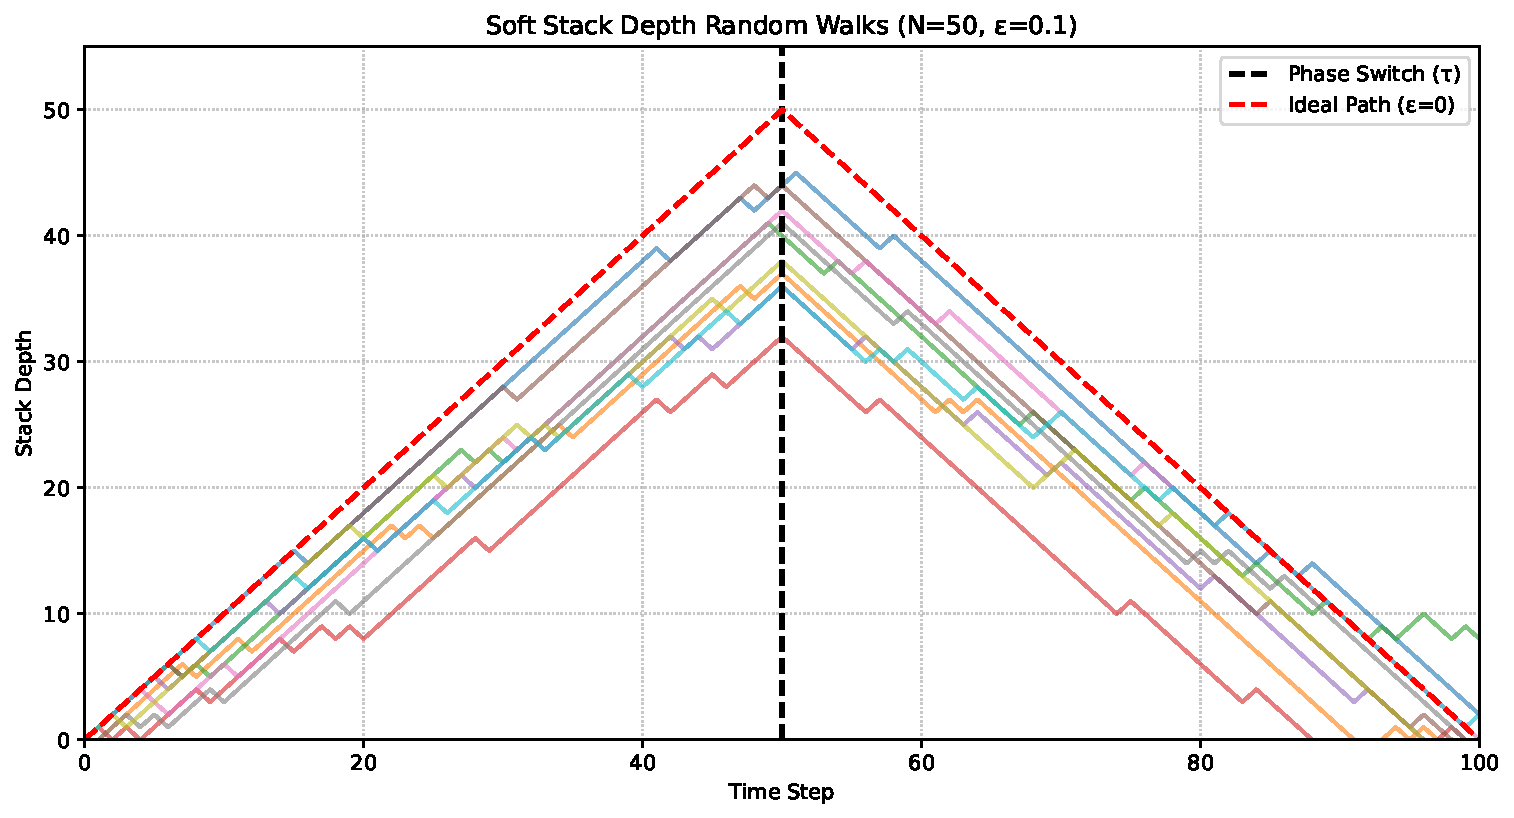
\includegraphics[width=0.8\linewidth]{figs/stack_random_walk_50_0.1.pdf}
    \caption{Caption}
    \label{fig:stackrw}
\end{figure}


\subsection*{Validation of the Upper Bound}
\begin{figure}
    \centering
    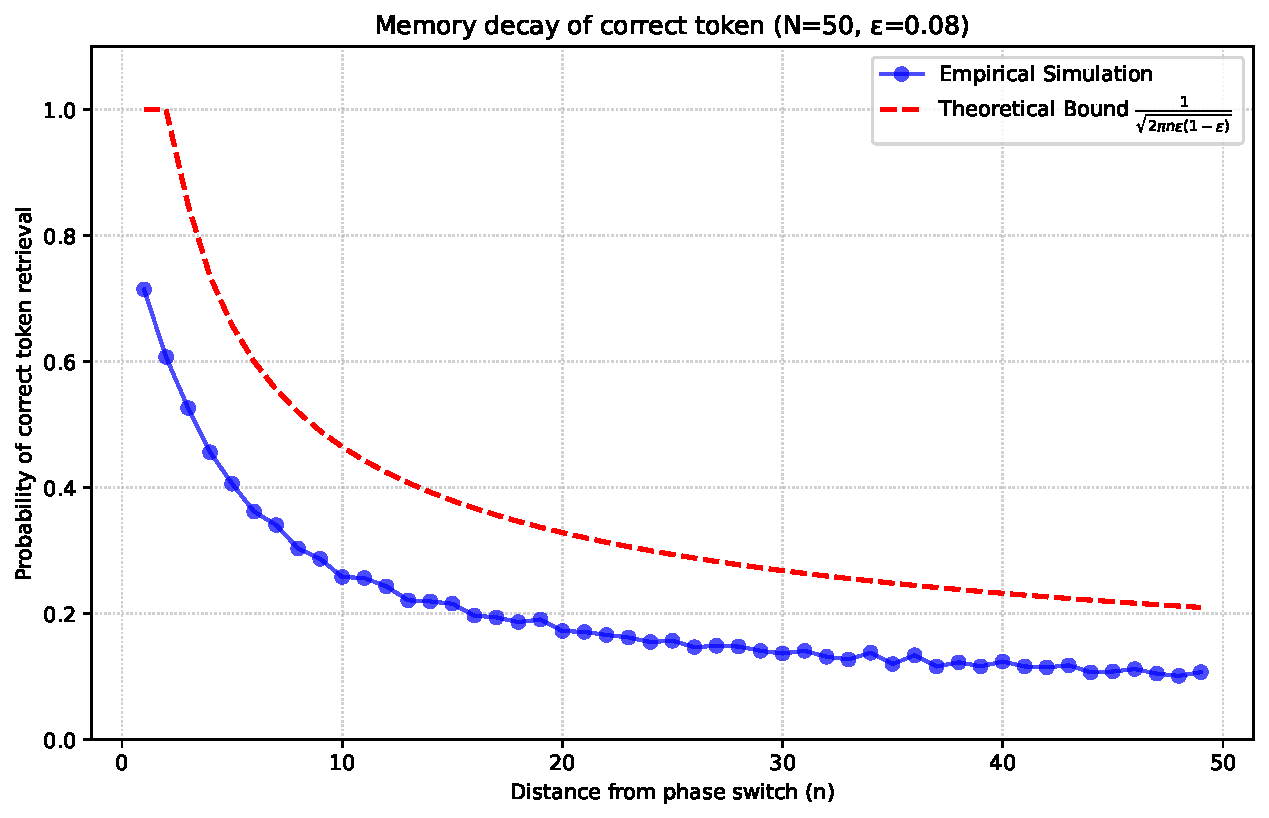
\includegraphics[width=0.8\linewidth]{figs/binary_stack_decay_50_0.08.pdf}
    \caption{Caption}
    \label{fig:memfid}
\end{figure}





\subsection*{Convergence to Random Guessing}

\begin{figure}
    \centering
    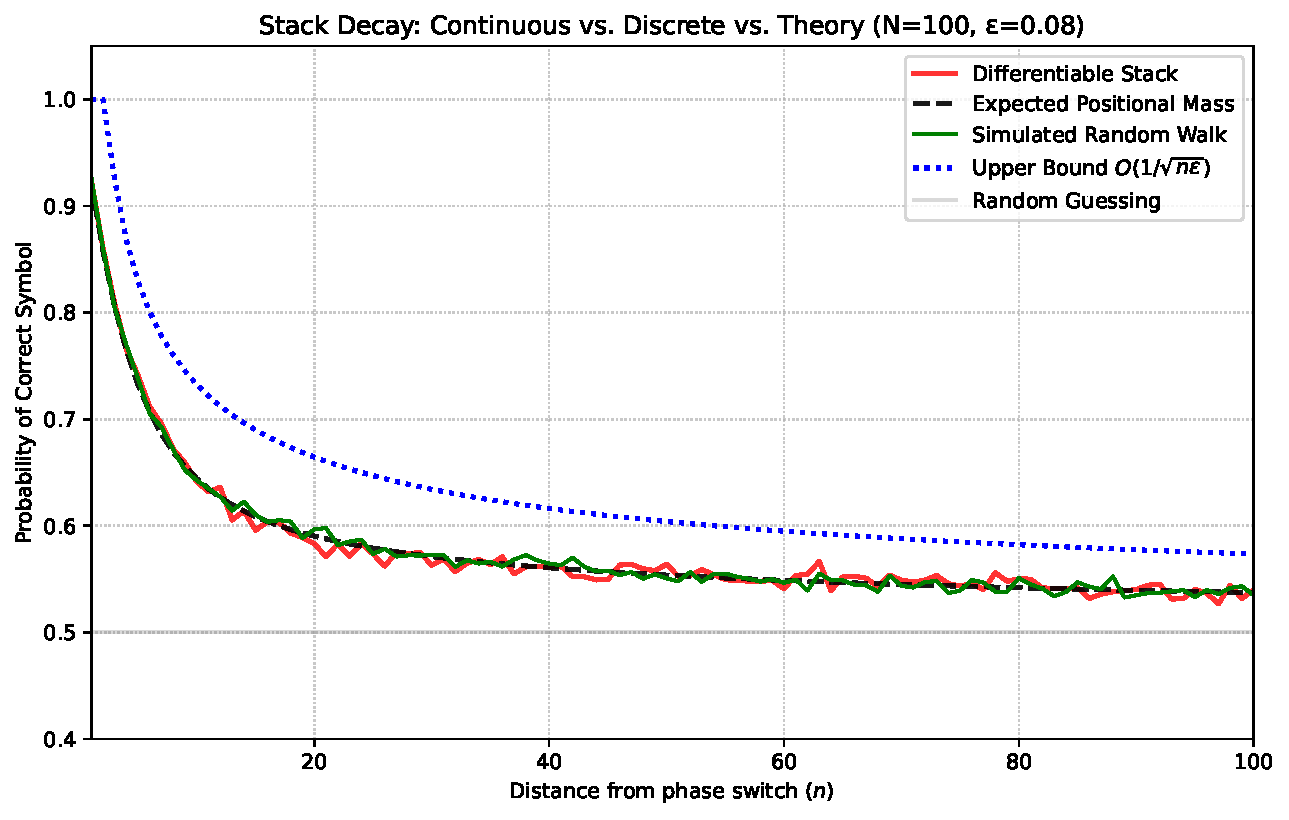
\includegraphics[width=0.8\linewidth]{figs/stack_decay_true_rw_simulation_100_0.08.pdf}
    \caption{Caption}
    \label{fig:randomguess}
\end{figure}



\section{Plots from trained model}


\begin{figure}[htbp]
    \centering
    \begin{minipage}{0.48\textwidth}
        \centering
        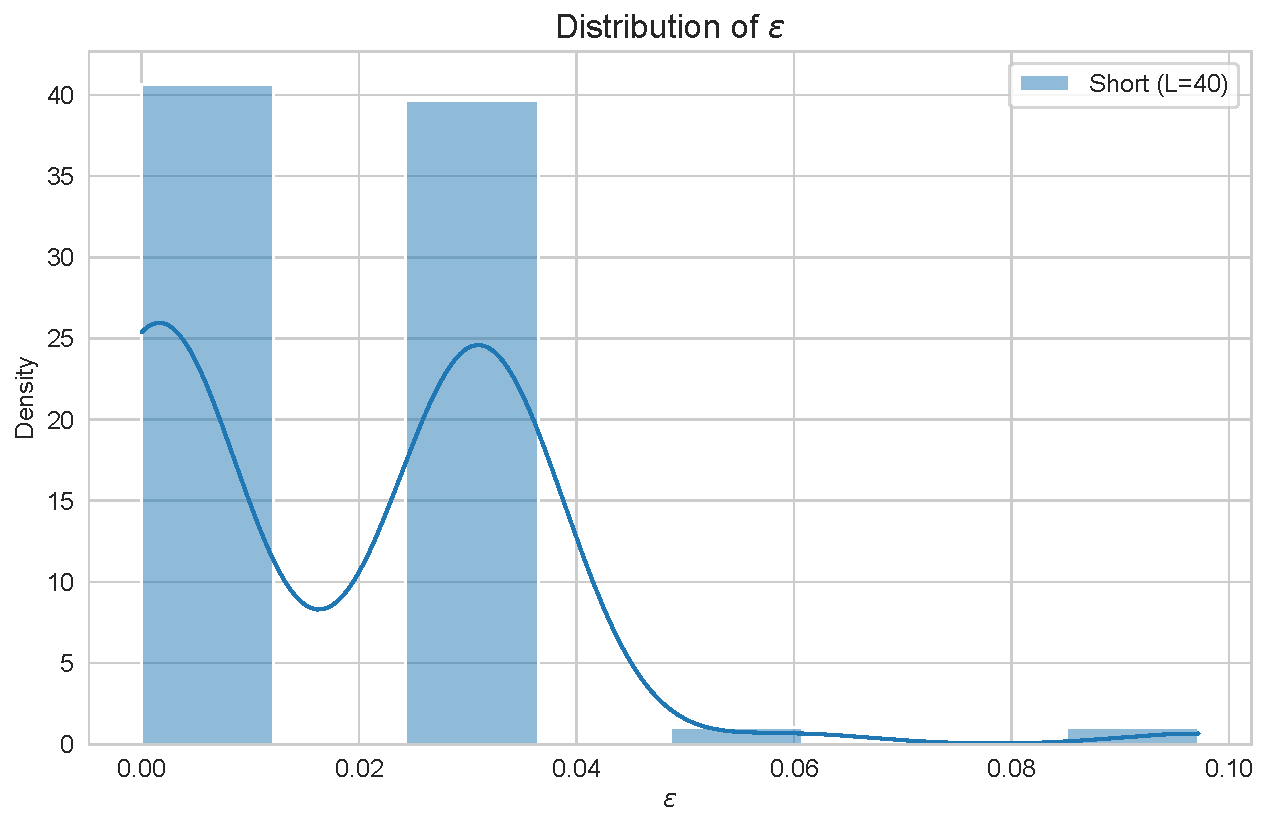
\includegraphics[width=\linewidth]{figs/epsilon_distribution_comparison_short.pdf} 
    \end{minipage}\hfill
    \begin{minipage}{0.48\textwidth}
        \centering
        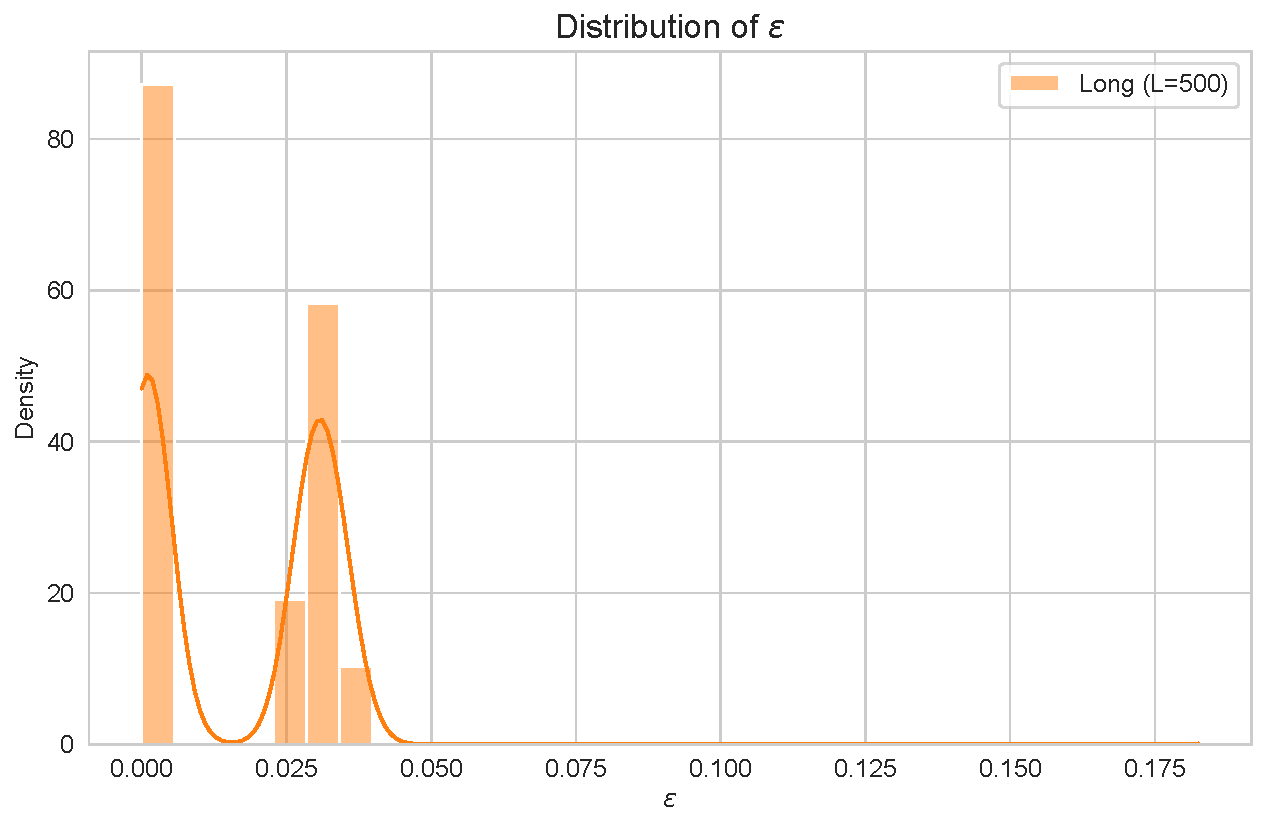
\includegraphics[width=\linewidth]{figs/epsilon_distribution_comparison_long.pdf} 
    \end{minipage}
    \caption{}
    \label{fig:eps_distribution}
\end{figure}


\begin{figure}
    \centering
    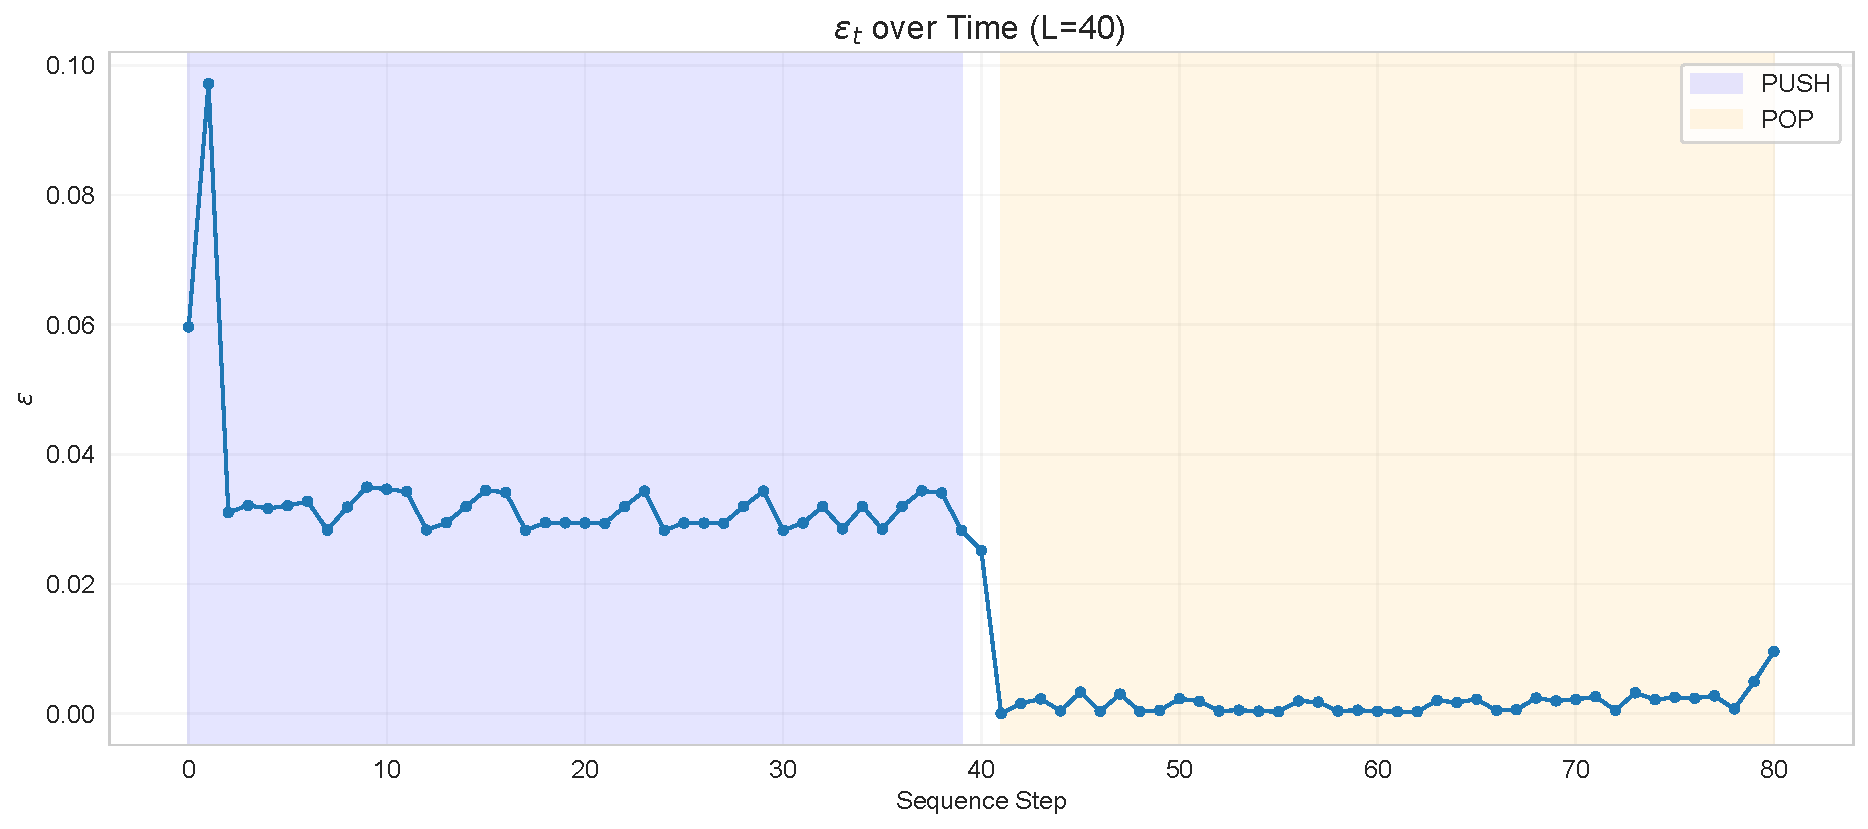
\includegraphics[width=0.8\linewidth]{figs/epsilon_time_short_plus.pdf}
    \caption{Caption}
    \label{fig:placeholder}
\end{figure}

\begin{figure}
    \centering
    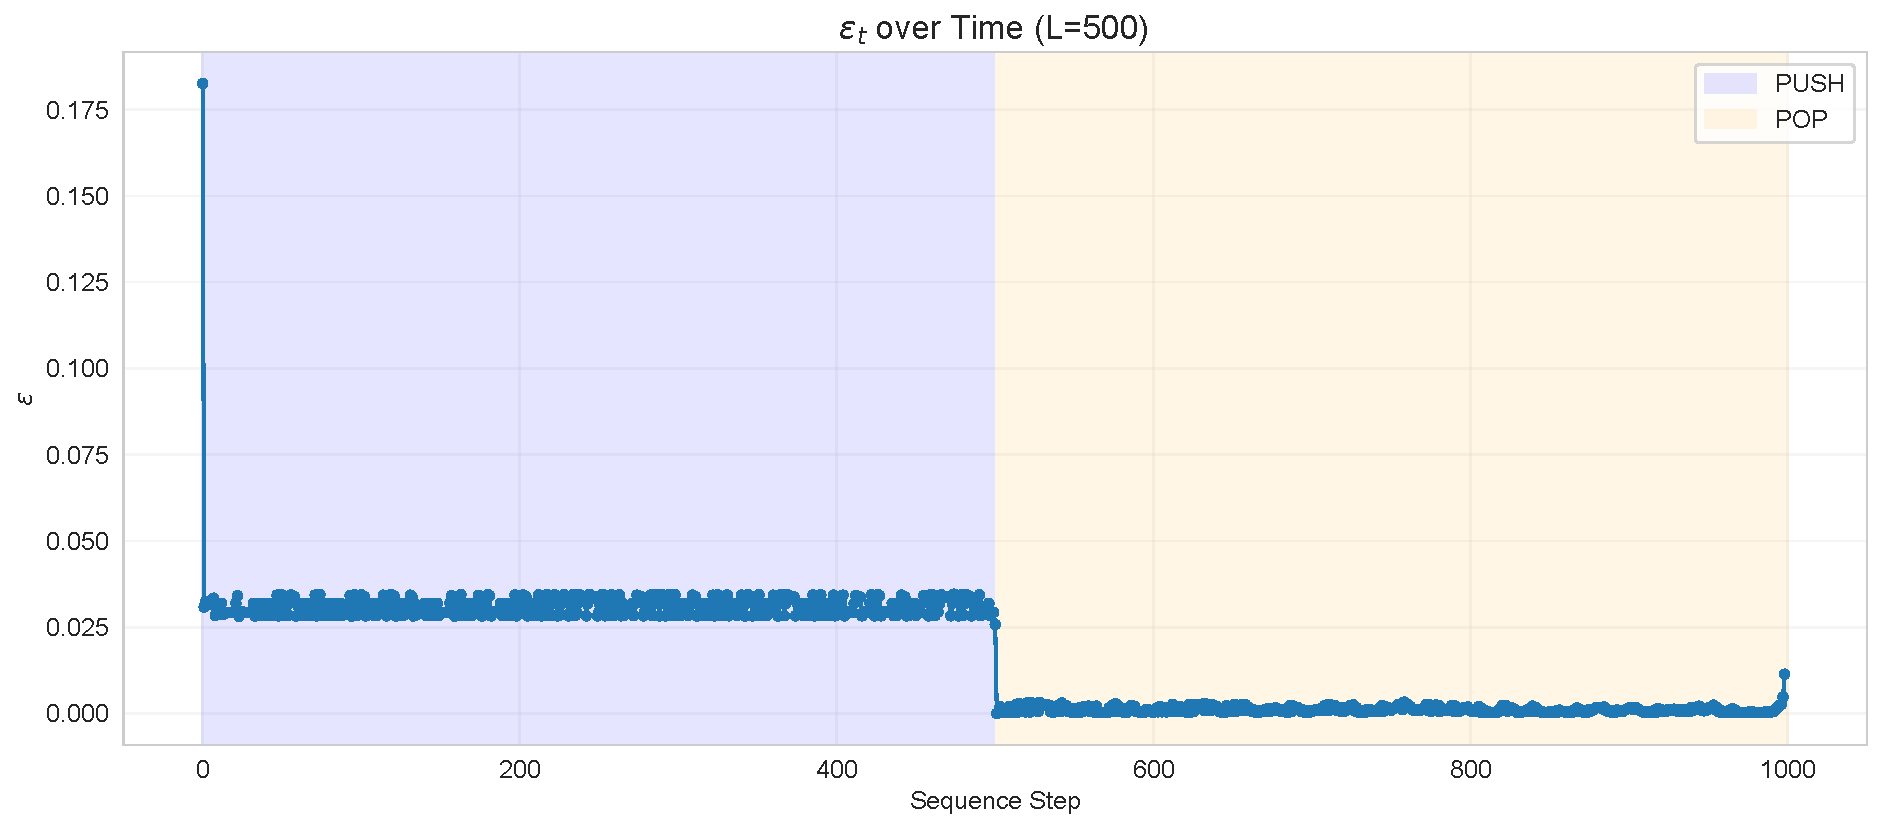
\includegraphics[width=0.8\linewidth]{figs/epsilon_time_long_plus.pdf}
    \caption{Caption}
    \label{fig:placeholder}
\end{figure}


\section{Open questions}

\begin{itemize}
    \item why binary string reversal?
    \item what statistics could one compute from any controller model to estimate in some sense its $\eps_t$ characteristics and hence predict its length gen failure due to memory fidelity. The nicest example would probably that uses the in horizon training or generalization bound.
    \item can we use online statics, i.e. during inference we could measure and track the $\eps$ rates and then feed these into a dynamic program to give us online some notion of confidence based on our predictions due to memory fidelity.
    \item what are the prod and cons of removing the issues of the soft stack say just by hardening the stack actions? is this a good fix?
\end{itemize}

\bibpunct{(}{)}{;}{a}{,}{;}
\bibliographystyle{chicago}
\setlength{\bibsep}{1pt}
\bibliography{references}

\end{document}
